



\subsection{Training}

In the VQA model on the new questions with 50 epochs. In particular, train the LSTM with attention on the visual features, and use a pre-trained CNN for encoding visual features. The pre-trained CNN we use is one proposed by the researchers in habitat-platform and could be found on EQA gihub page.\footnote{ Link to the code for running the VQA baseline model. The same page include an attachment to the pre-trianed-CNN "\url{https://github.com/facebookresearch/habitat-lab/tree/master/habitat_baselines/il\#eqa-cnn-pretrain-model}.} 

We pick the model trained on the last epoch. The model has 1.10 average loss and  0.79 average accuracy. %, 2.21. % average mean rank, and 0.73 average reciprocal rank. 


\subsection{Evaluating}


The overall evaluation on the validation set with all the question types show an average accuracy of 0.61 and average loss 2.10. However, the accuracy score is by no means indicating a good system performance. As mentioned earlier, VQA system could cheat its ways by remembering answers and score high in accuracy results. These scores are attributed to a great extent to the bias we have in the size questions, where most of the answers to size questions are "medium". The absolute bias in the size question contribute to a higher score in the average accuracy of the overall validation. 


The results of the size questions showed all the predictions to be of 'medium' answer. In figure \ref{fig:heatmapSize}, the illustration of the predictions shows that all the answers to size questions been predicted as "medium". The results of the evaluation of the size questions are not surprising given the significant imbalance in their answer distribution. 


\begin{figure}[H]
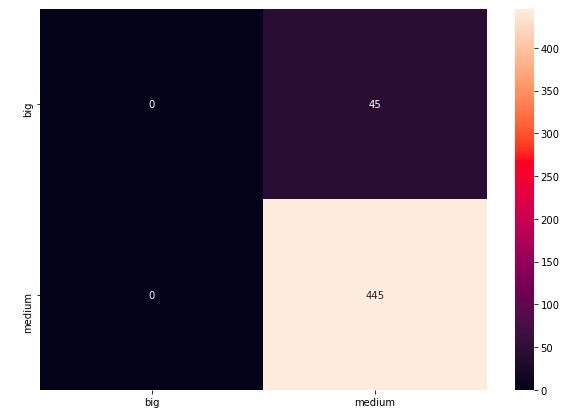
\includegraphics[scale=0.3]{images/heatmapSize.png}
\caption{A map shows the number of predictions for each question type sorted by answer. All answers for size questions were predicted "medium". The row an column with big categories are zero}
\label{fig:heatmapSize}
\end{figure}



A reliable measure of evaluation for spatial questions is measuring the performance on the questions of "no" answers. The bias to 'yes' answers  in spatial questions was an intended learning experiment, and it is predictable that the system would preform well in predicting the questions with 'yes' answer. However, the extent in which the model's predictions are  based on exploiting bias could be measure by how many questions with "no" answer have been predicted correctly. Otherwise, given the bias of the answers to "yes", an indicator of learning shortcomings would be the number of times the model answered 'yes' to a question with 'no' answer. A positive learning indicator is the number of times that the system  predicted question with 'no' answer correctly. The system's prediction to questions with 'no' answer, therefore, provides a good validation measurement to how well the VQA model learnt about spatial relations. 



  

\begin{figure}[H]
 \centering
\subfloat[label 1]{{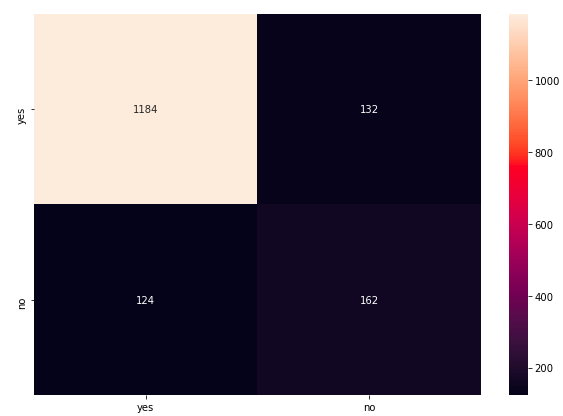
\includegraphics[width=5cm]{images/heatmapSpa.png} \label{<figure1>}}}
\subfloat[label 2]{{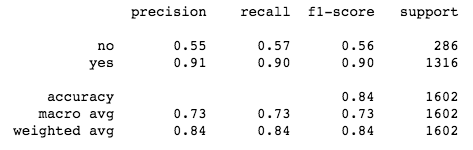
\includegraphics[width=5cm]{images/SpScores.png}\label{<figure2>} }}

\caption{A map shows the number of predictions for each question type sorted by answer.}
\end{figure}




In the section below we see the difference in the distribution of answer-predictions of the color questions between the original model and the model after being trained on the new questions. 

\begin{figure}[H]
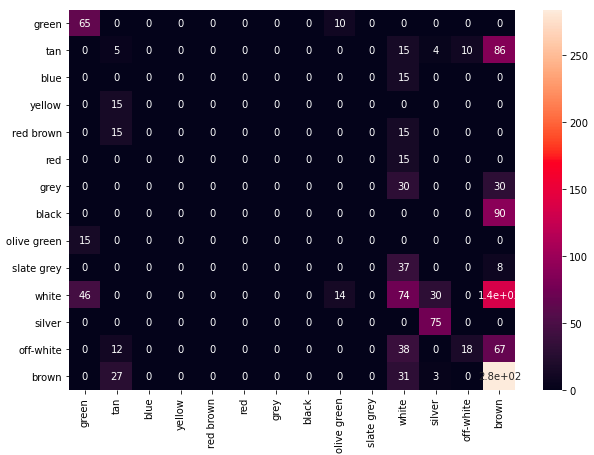
\includegraphics[scale=0.45]{images/Heatmapbefore.png}
\label{fig:Heatmapbefore}
\caption{Predictions of color questions for the original model, untrained with new questions}
\end{figure}

\begin{figure}[H]
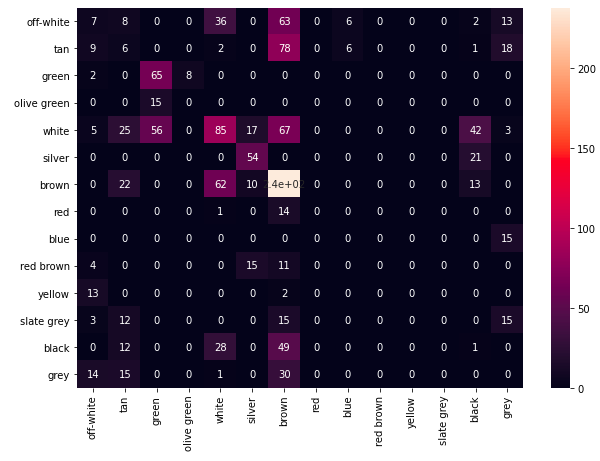
\includegraphics[scale=0.45]{images/HeatmapAfter.png}
\label{fig:HeatmapAfter}
\caption{Predictions of color questions on the model trained with new questions}
\end{figure}





\subsection{Discussion}

We should treat neural models as a theory or brain that is applicable and functional for every task scenario \cite{regier1996human}  

\cite{dobnik2009teaching}

Hcolor questions could get more complex as "people employ compositional color descriptions to express meanings not covered by basic terms, such as greenish-blue" \cite{monroe2016learning}. It would be shallow to assume that color questions are simplistic, especially if we expect the system to answer colors beyond the basic color terms like "green" and "red." 

\cite{monroe2017colors}


intersective compostionality: intersective compositionality is when two words which one is attributed to the meaning of the other "brown bear" where it means a bear that is brown-[brown and bear] 

non-intersective compostionality: non-intersective is one word does not modify the second, such as [Teddy bear]. 'Teddy bear' cannot be mean a bear that is 'Teddy', 'Teddy' is not an attribute of a bear so not [Teddy + bear]. Teddy + bear is instead a different entity with a different perceptual meaning. \cite{larsson-2017-compositionality} 

